\subsection{Is the sampling window long enough? Equilibration and an equilibrium reference}\label{sec:results-equil}
The protocol discards $\EfiveBurn$ sweeps and samples $\EfiveSample$ (\cref{sec:protocol}), and the estimator uses the variance of the energy in that window. Two diagnostics ask whether that window is adequate, and whether any inadequacy explains the dilute offset.

\paragraph{E9a: single long traces.} For $\EnineaCases$ cells ($N\in\{64,100\}$, one trace each, $\EnineaTotalSweeps$ sweeps from a random start; seed fixed) we compare the sampling window with late windows of the same length and with the long-run variance. \Cref{tab:E9a} lists the offset of the protocol-window mean from the late mean in units of the long-run standard deviation, and the ratio of the protocol-window variance to the long-run variance. The ratio ranges from $\EnineaRatioMin$ to $\EnineaRatioMax$ (median $\EnineaRatioMedian$); in $\EnineaBelowHalf$ of $\EnineaCases$ cells it is below $1/2$, and the mean offset exceeds one standard deviation in $\EnineaOffGtOne$ cells (maximum $\EnineaOffMax$). The window is therefore not equilibrated in every cell, notably at low temperature and dilute composition, and its variance is on the whole biased low and noisy. Each cell has a single trace, so the table documents the effect without estimating its distribution.

\begin{table}[t]
\centering\small
\caption{E9a. Protocol window (sweeps 500--800) versus late windows (sweeps 20\,000--40\,000) of one trace per cell. Offset: protocol mean minus late mean, in units of the long-run standard deviation of $E$. $V_{\rm prot}$, $V_{\rm late}$: variance of $E$ in the two windows; the last column is their ratio.}\label{tab:E9a}
\begin{tabular}{rrrrrrr}
\toprule
$N$ & $f$ & $T$ & offset & $V_{\rm prot}$ & $V_{\rm late}$ & ratio\\
\midrule
64 & 0.05 & 1.8 & +2.1 & 1480 & 8449 & 0.18 \\
64 & 0.05 & 2 & +0.3 & 1601 & 2890 & 0.55 \\
64 & 0.05 & 2.2 & -0.0 & 1708 & 1805 & 0.95 \\
64 & 0.20 & 2 & +1.3 & 9158 & 12395 & 0.74 \\
64 & 0.20 & 2.2 & -0.1 & 10308 & 21325 & 0.48 \\
64 & 0.20 & 2.4 & -0.1 & 18921 & 13995 & 1.35 \\
64 & 0.50 & 2.2 & +0.6 & 7019 & 24157 & 0.29 \\
64 & 0.50 & 2.4 & +0.4 & 23346 & 25216 & 0.93 \\
64 & 0.50 & 2.6 & +0.2 & 12048 & 18754 & 0.64 \\
100 & 0.05 & 1.8 & +2.3 & 4353 & 17198 & 0.25 \\
100 & 0.05 & 2 & +0.2 & 4910 & 8747 & 0.56\\
\bottomrule
\end{tabular}
\end{table}

\paragraph{E9b: equilibrium reference.} To separate the effect of the short window from the finite-size behaviour of the estimator, we re-ran six $(N,f)$ systems on the temperature grid $1.5\le T\le2.8$ in steps of $0.05$ with $10\,000$ burn-in sweeps and $50\,000$ sampling sweeps, using $3$ replicates for $N=32$ and $2$ for $N=64$ ($\EninebRuns$ runs in total). The integrated autocorrelation time of the energy (Sokal windowing) has median $\EninebTauMedian$ sweeps over all runs and maximum $\EninebTauMax$ sweeps; the maximum is more than ten times the 300-sweep window, so the window is shorter than $\tau_{\rm int}$ in the worst cells.

\Cref{tab:E9b} and \cref{fig:equilibrium} report the temperature of the peak of the replicate-mean variance under the long run, the range of the per-replicate peaks, the peak of the specific heat $\mathrm{Var}(E)/(N^2T^2)$, and the corresponding peak of the original protocol of E5, next to the exact binodal $\Tb(f)$.

\begin{table}[t]
\centering\small
\caption{E9b. Variance-peak temperature under the long equilibrium protocol versus the exact binodal. $\Tb$: exact binodal; $\hat T_{\rm eq}$: peak of the replicate-mean $\mathrm{Var}(E)$; range: smallest--largest per-replicate peak; $\hat T_C$: peak of the replicate-mean specific heat; $\hat T_{\rm prot}$: peak of the mean variance under the 300-sweep protocol (E5); $\tau$: mean $\tau_{\rm int}$ (sweeps) at $\hat T_{\rm eq}$. Grid step $0.05$.}\label{tab:E9b}
\begin{tabular}{rrrrrrrr}
\toprule
$N$ & $f$ & $\Tb$ & $\hat T_{\rm eq}$ & range & $\hat T_C$ & $\hat T_{\rm prot}$ & $\tau$\\
\midrule
32 & 0.05 & 2.032 & 1.75 & 1.75--1.75 & 1.65 & 1.80 & 80 \\
32 & 0.10 & 2.188 & 2.00 & 1.95--2.00 & 1.90 & 2.15 & 59 \\
32 & 0.20 & 2.261 & 2.15 & 2.15--2.20 & 2.15 & 2.30 & 48 \\
32 & 0.50 & 2.269 & 2.40 & 2.35--2.40 & 2.20 & 2.70 & 21 \\
64 & 0.05 & 2.032 & 1.85 & 1.85--1.85 & 1.85 & 1.70 & 258 \\
64 & 0.50 & 2.269 & 2.30 & 2.25--2.30 & 2.30 & 2.40 & 87\\
\bottomrule
\end{tabular}
\end{table}

\begin{figure}[t]
\centering
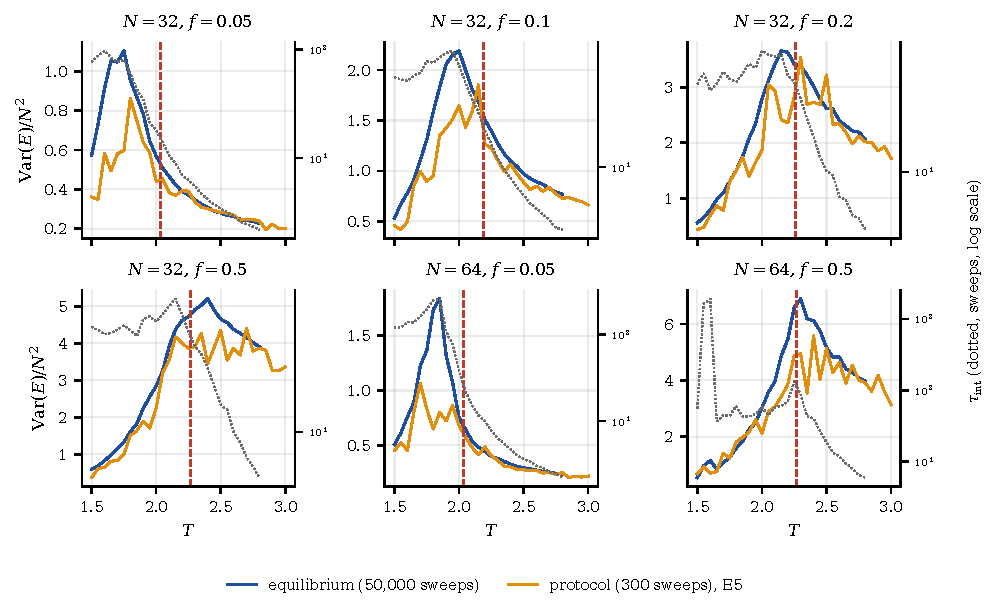
\includegraphics[width=\linewidth]{figures/fig_equilibrium.pdf}
\caption{E9b. $\mathrm{Var}(E)/N^2$ versus $T$ under the long equilibrium protocol (blue) and the 300-sweep protocol of E5 (orange); dashed vertical line: exact binodal; dotted: $\tau_{\rm int}$ on a logarithmic axis (right).}\label{fig:equilibrium}
\end{figure}

We read \cref{tab:E9b} with its limits in mind: a $0.05$ grid and two or three replicates.
(i) The protocol and equilibrium peaks differ by at most $0.30$ in $T$ (largest at $N=32$, $f=0.5$). The window effect seen in E9a moves the estimate by a few grid steps; it does not explain the dilute offsets of \cref{sec:results-demix}.
(ii) For $f=0.05$ the equilibrium peak lies below $\Tb$ ($1.75$ versus $2.032$ at $N=32$, $1.85$ versus $2.032$ at $N=64$); at $f=0.10$ and $0.20$ at $N=32$ it lies $0.19$ and $0.11$ below. The gap at $f=0.05$ is smaller at $N=64$ than at $N=32$, but the $N=64$ peaks come from two replicates on a coarse grid, so all we can say is that the data do not contradict a decreasing offset. The direction agrees with finite-size droplet formation \citep{binder1987,biskup2002}; we did not test the scaling.
(iii) At $f=0.5$ the equilibrium peak lies above the critical temperature ($2.40$ at $N=32$, $2.30$ at $N=64$ versus $\Tc=2.269$), consistent with a finite-size shift towards $\Tc$ from above as $N$ grows.
The variance peak is a finite-size quantity. Its location depends on $N$ and, in part, on the window length, and it should not be identified with $\Tb$ without a finite-size analysis.
